\begin{figure*}[p]
\centering
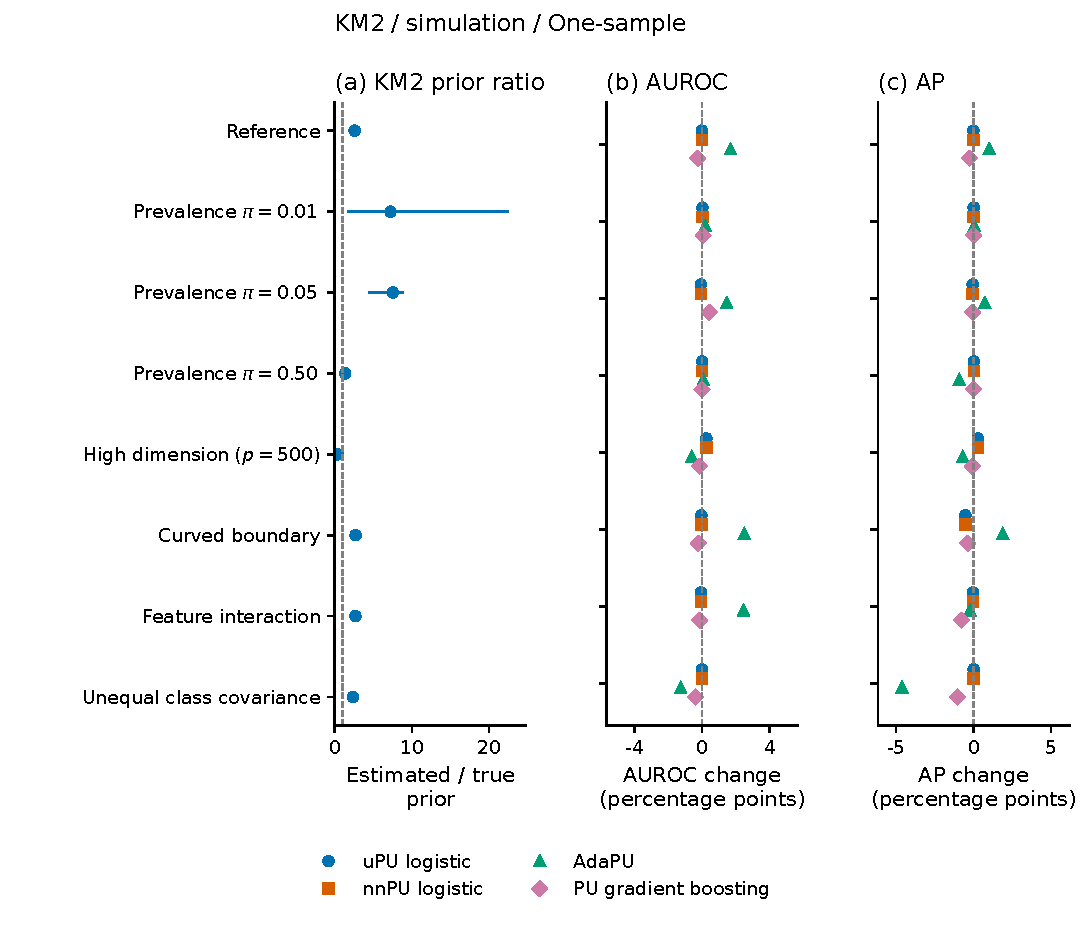
\includegraphics[page=1,width=\textwidth]{revised_figures/fig_s_estimated_prior.pdf}
\caption{KM2 estimated-prior diagnostic, specific to the estimator and implementation audited in estimated-prior experiment. Prior panels show the mean estimated/true prior ratio and empirical 5th--95th percentiles across repetitions; performance panels show paired mean changes from the correct supplied prior, in percentage points. The table retains every audited setting and real-data budget for the four directly prior-dependent fitted methods. Simulation cases use 100 repetitions; real-data cases use 20 repeated splits, whose uncertainty is conditional resampling uncertainty rather than independent-population Monte Carlo uncertainty. KM2 findings are not generalized to other prior estimators. Simulation / One-sample. Performance panels show paired means. The accompanying table and numeric CSV retain uncertainty and case counts. Prior whiskers are empirical 5th--95th percentiles, not confidence intervals.}
\label{fig:s-estimated-prior-1}
\end{figure*}
\begin{figure*}[p]
\centering
\includegraphics[page=2,width=\textwidth]{revised_figures/fig_s_estimated_prior.pdf}
\caption{KM2 estimated-prior diagnostic, specific to the estimator and implementation audited in estimated-prior experiment. Prior panels show the mean estimated/true prior ratio and empirical 5th--95th percentiles across repetitions; performance panels show paired mean changes from the correct supplied prior, in percentage points. The table retains every audited setting and real-data budget for the four directly prior-dependent fitted methods. Simulation cases use 100 repetitions; real-data cases use 20 repeated splits, whose uncertainty is conditional resampling uncertainty rather than independent-population Monte Carlo uncertainty. KM2 findings are not generalized to other prior estimators. Simulation / Two-sample. Performance panels show paired means. The accompanying table and numeric CSV retain uncertainty and case counts. Prior whiskers are empirical 5th--95th percentiles, not confidence intervals.}
\label{fig:s-estimated-prior-2}
\end{figure*}
\begin{figure*}[p]
\centering
\includegraphics[page=3,width=\textwidth]{revised_figures/fig_s_estimated_prior.pdf}
\caption{KM2 estimated-prior diagnostic, specific to the estimator and implementation audited in estimated-prior experiment. Prior panels show the mean estimated/true prior ratio and empirical 5th--95th percentiles across repetitions; performance panels show paired mean changes from the correct supplied prior, in percentage points. The table retains every audited setting and real-data budget for the four directly prior-dependent fitted methods. Simulation cases use 100 repetitions; real-data cases use 20 repeated splits, whose uncertainty is conditional resampling uncertainty rather than independent-population Monte Carlo uncertainty. KM2 findings are not generalized to other prior estimators. Real data / One-sample / budget 0.05. Performance panels show paired means. The accompanying table and numeric CSV retain uncertainty and case counts. Prior whiskers are empirical 5th--95th percentiles, not confidence intervals.}
\label{fig:s-estimated-prior-3}
\end{figure*}
\begin{figure*}[p]
\centering
\includegraphics[page=4,width=\textwidth]{revised_figures/fig_s_estimated_prior.pdf}
\caption{KM2 estimated-prior diagnostic, specific to the estimator and implementation audited in estimated-prior experiment. Prior panels show the mean estimated/true prior ratio and empirical 5th--95th percentiles across repetitions; performance panels show paired mean changes from the correct supplied prior, in percentage points. The table retains every audited setting and real-data budget for the four directly prior-dependent fitted methods. Simulation cases use 100 repetitions; real-data cases use 20 repeated splits, whose uncertainty is conditional resampling uncertainty rather than independent-population Monte Carlo uncertainty. KM2 findings are not generalized to other prior estimators. Real data / One-sample / budget 0.20. Performance panels show paired means. The accompanying table and numeric CSV retain uncertainty and case counts. Prior whiskers are empirical 5th--95th percentiles, not confidence intervals.}
\label{fig:s-estimated-prior-4}
\end{figure*}
\begin{figure*}[p]
\centering
\includegraphics[page=5,width=\textwidth]{revised_figures/fig_s_estimated_prior.pdf}
\caption{KM2 estimated-prior diagnostic, specific to the estimator and implementation audited in estimated-prior experiment. Prior panels show the mean estimated/true prior ratio and empirical 5th--95th percentiles across repetitions; performance panels show paired mean changes from the correct supplied prior, in percentage points. The table retains every audited setting and real-data budget for the four directly prior-dependent fitted methods. Simulation cases use 100 repetitions; real-data cases use 20 repeated splits, whose uncertainty is conditional resampling uncertainty rather than independent-population Monte Carlo uncertainty. KM2 findings are not generalized to other prior estimators. Real data / Two-sample / budget 0.05. Performance panels show paired means. The accompanying table and numeric CSV retain uncertainty and case counts. Prior whiskers are empirical 5th--95th percentiles, not confidence intervals.}
\label{fig:s-estimated-prior-5}
\end{figure*}
\begin{figure*}[p]
\centering
\includegraphics[page=6,width=\textwidth]{revised_figures/fig_s_estimated_prior.pdf}
\caption{KM2 estimated-prior diagnostic, specific to the estimator and implementation audited in estimated-prior experiment. Prior panels show the mean estimated/true prior ratio and empirical 5th--95th percentiles across repetitions; performance panels show paired mean changes from the correct supplied prior, in percentage points. The table retains every audited setting and real-data budget for the four directly prior-dependent fitted methods. Simulation cases use 100 repetitions; real-data cases use 20 repeated splits, whose uncertainty is conditional resampling uncertainty rather than independent-population Monte Carlo uncertainty. KM2 findings are not generalized to other prior estimators. Real data / Two-sample / budget 0.20. Performance panels show paired means. The accompanying table and numeric CSV retain uncertainty and case counts. Prior whiskers are empirical 5th--95th percentiles, not confidence intervals.}
\label{fig:s-estimated-prior-6}
\end{figure*}
